\chapter{Thermal conductivity simulations of Silica glass}  \label{ch:silica}

%\LEnote{Thermal conductivity simulations for Silica glasses??}

The calculation of the lattice thermal conductivity of a material using equilibrium MD simulations requires an accurate knowledge of the interatomic interactions, a sample of adequate \emph{size}, and a sufficient \emph{simulation length}. 
A good interatomic force field should faithfully reproduce the structural and dynamical properties of the material, as both will be important to correctly predict the thermal conductivity. 
An adequately large size is required to account for all the vibrational contributions to heat transport: if the system is too small, the long-wavelength modes will be neglected or severely affected, thus altering the value of thermal conductivity estimated via the GK equation. 
A sufficiently long simulation is needed to let the GK estimate converge within a target statistically accuracy. 

The simulation of amorphous systems such as silica glass, though, presents additional challenges. The structure of an amorphous solid is a non-equilibrium configuration, with extremely long relaxation times. 
In order to generate it, one can perform a virtual \emph{quenching} experiment: the system is melted at high temperature and then cooled gradually down to a target temperature, where it is then equilibrated and data can be collected. 
This procedure is in all respects a simulated annealing experiment looking for the most stable configuration in an extremely rough free energy landscape. 
The quenching protocol adopted will affect the final structural and vibrational properties of the sample, hence we expect the thermal conductivity to be affected by its details as well. 

Very few studies have attempted to compute the thermal conductivity of a-SiO$_2$ with classical MD simulations and no \abinitio study has ever been performed. Almost all of the existing simulations were carried out with non-equilibrium methods, where strong finite-size effects are accounted for with difficulty, whereas only one of them was performed at equilibrium via the GK equation. 
These facts demonstrate the practical difficulties involved in the numerical estimation of $\kappa$ and the lack of a reliable method to do so, as we discussed in Chapter~\ref{ch:data-analysis}. 

%The simulation of an amorphous system such as a-SiO$_2$ with classical MD and the estimation of its thermal conductivity require a few ingredients. 
%First of all, we need a good interatomic force field that faithfully reproduces the structural and dynamical properties of the glass. Both will be important to correctly predict the thermal conductivity.
%and will be briefly discussed in Sec.~\ref{sec:silica-force-field}.
%Second, we need to choose a system size and generate the amorphous structure, a process that is usually performed by melting and equilibrating the system at high temperatures, followed by a cooling phase in which it is gradually brought to the target temperature. At this point the system is equilibrated and data can start to be collected. 
%This ``quenching'' protocol also affects the final structural and vibrational properties of the sample, hence we expect the thermal conductivity to be affected by its details. We shall introduce both these points in Section~\ref{sec:silica-classical} of this chapter. 

In this chapter we apply the \abinitio GK theory and many of the methods discussed in the previous chapters to the calculation of the thermal conductivity of silica glass. 
In Section~\ref{sec:silica-state-of-the-art} we review the classical and \abinitio studies of a-SiO$_2$ available in the literature, pointing out how the force field, the sample size, and the preparation protocol affect its structural, vibrational, and thermal properties. 
We find that although the structural properties are described fairly well by classical potentials, the vibrational properties are poorly accounted for and thus call for an \abinitio approach. 
In Section~\ref{sec:results-classical}, we use classical simulations to study the dependence of the computed thermal conductivity on many of the simulation details, such as the sample size and quenching protocol, and to determine the feasibility of \abinitio simulations. 
In Section~\ref{sec:results-quantum}, we choose one sample of silica and we simulate it with Car-Parrinello MD at four different temperatures. The trajectories thus generated are used to compute the \abinitio heat flux and the GK thermal conductivity, making use of many of the concepts and techniques discussed so far. Finally, we compare our classical and \abinitio results with experiments. 

%All this classical study will be instrumental in determining the feasibility of \abinitio calculations of thermal conductivity of a-SiO$_2$, using the DFT formulation of the heat flux that was presented in Chapter~\ref{ch:dft-heat}. One classical sample will be selected and simulated with Car-Parrinello MD at four different temperatures. The simulation details and results will be presented in Sec.~\ref{sec:results-quantum}.


%%%%%%%%%%%%%%%%%%%%%%%%%%%%%%%%%%%%%%%%%%%%%%%%%%%%%%%%%%%%%%%%%%%%%%%%%
\section{State of the art}  \label{sec:silica-state-of-the-art}

\subsection{BKS force field}  \label{sec:silica-force-field}
%\LEnote{* FIGURA? *}
The structure of amorphous silica is made of SiO$_4$ tetrahedral units, where silicon is at the center, bonded to 4 oxygen atoms located at the vertices. Each oxygen, in turn, bridges the tetrahedral vertices, thus bonding between two silicon centers. The variation in orientation of adjacent tetrahedra makes the medium- and long-range structures disordered, forming a typical glass network.

One of the most successful and broadly adopted force fields for a-SiO$_2$ is the so-called BKS potential \cite{Silica-BKS-1990}. 
The BKS potential is a two-body potential devised by \citeauthor*{Silica-BKS-1990} who fitted self-consistent-field Hartree-Fock calculations on small silica clusters, and it is defined as the sum of a Coulomb and a Buckingham potential:
\begin{equation}
    v_{\alpha\beta}^{\mathrm{BKS}}(R) = \mathtt{e}^2 \frac{q_\alpha q_\beta}{R} + A_{\alpha\beta}\mathrm{e}^{-B_{\alpha\beta}R} - \frac{C_{\alpha\beta}}{R^6}, \label{eq:BKS}
\end{equation}
where $\alpha,\beta \in [\text{Si},\text{O}]$, and $R$ is the distance between the ions $\alpha$ and $\beta$. 

Despite its simplicity, BKS was showed to predict remarkably well many properties of SiO$_2$, among which its complicated phase diagram \cite{Saika2004}. 
Other force fields have been used in the literature, ranging from re-parametrizations of the BKS potential \cite{Carre2008}, to polarizable force fields (\emph{e.g.} \citet{Tangney2002}) and reactive ones (\emph{e.g.} ReaxFF \cite{Yuan2001}). 
Notwithstanding, the BKS potential is still the mostly adopted force field in classical simulations of a-SiO$_2$, thanks to its ability to generate very good glass structures. 
In the following, and partly in Sec.~\ref{sec:silica-quenching}, we are going to summarize how well the properties of amorphous silica are described by this potential and others.


\paragraph{Structural properties}
Si-O bonds are generally considered to have partial ionic and covalent character. The BKS potential is spherical, therefore it does not describe the directional nature of the covalent bond, but it can anyway achieve the tetrahedral structure through a strictly repulsive interaction between oxygen atoms. We can expect that the bond's directionality could be better described by other more sophisticated potentials or by \abinitio methods, yet the BKS' abilities in predicting the amorphous structure of silica glass are very remarkable. 
For example, \citet{Tian2017} compared the structures of silica obtained from different force fields, \emph{e.g.} BKS and ReaxFF. They quenched a fully melted silica box of density $\rho=2.2\un{g/cm^3}$ from $5000\un{K}$ to $300\un{K}$ at $5\times 10^{12}\un{K/s}$ in the NVT ensemble. 
The BKS and ReaxFF potentials both generate realistic silica structures \cite{Vollmayr1996,Yuan2001}, with radial distribution functions, neutron structure factors, and coordination numbers that reasonably reproduce the experimental observations.
The radial distribution functions, in very good agreement with experiment, show a sharp peak corresponding to the Si-O bond length at $\sim 1.6\un{\angstrom}$, the peak corresponding to the O-O distance at $\sim 2.6\un{\angstrom}$, and the one corresponding to the Si-Si distance at $\sim 3.1\un{\angstrom}$. 
The coordination numbers can be used to detect coordination defects. By choosing a cutoff length for Si-O pairs of $\sim 2.15\un{\angstrom}$, BKS reproduces a realistic coordination environment for Si and O, with over $99.6\%$ of atoms being normally coordinated (4-fold Si and 2-fold O). ReaxFF, instead, tends to generate more coordination defects, with $\sim 97.5\%$ of normally coordinated atoms.
Nevertheless, the quenching process largely influences the macroscopic and microscopic properties of the generated glass, as we will comment diffusively later, in Sec.~\ref{sec:silica-quenching}. 


\paragraph{Vibrational properties}
\begin{figure}[!tb]
    \centering
    \subfigure[\label{fig:silica-vdos-classical}]{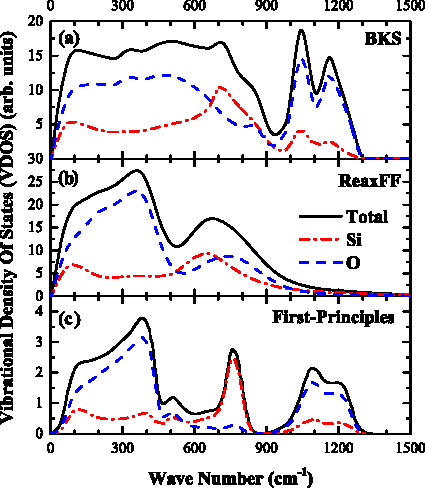
\includegraphics[width=7cm]{chapters/chapter6/figures/Tian_VDOS_silica.pdf}}
    \subfigure[\label{fig:silica-vdos-abinitio}]{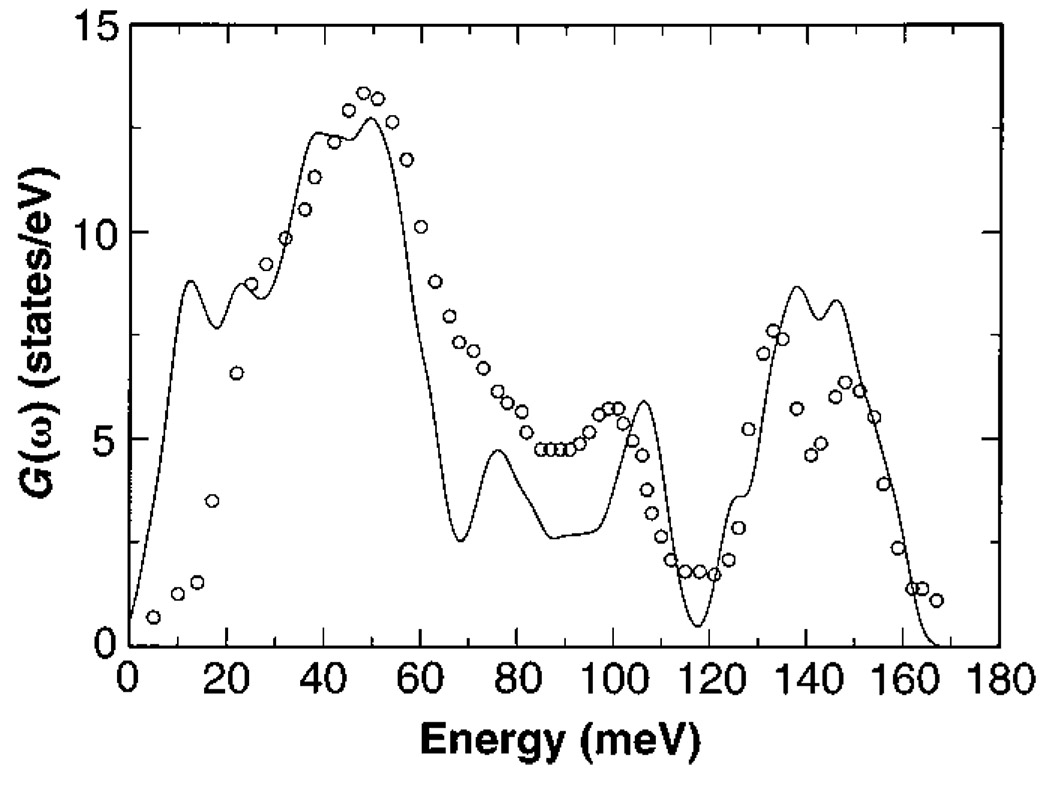
\includegraphics[width=6cm]{chapters/chapter6/figures/Sarnthein_Car_abinitio_VDOS_silica-2.jpg}}
    \caption{
    (a) Total and partial VDOS of a-SiO$_2$ computed for the BKS and ReaxFF, and compared with the first-principles results of \citet{Bhattarai2016}. Adapted from Ref.~\cite{Tian2017}.
    (b) Effective VDOS of an a-SiO$_2$ sample of $72$ atoms at experimental density $2.20\un{g/cm^3}$, computed from AI-CPMD simulations within the local density approximation (solid line) and compared to neutron scattering data (circles). Reproduced from Ref.~\cite{Sarnthein1997}.}
\end{figure}

Besides the structure of the generated sample, the thermal conductivity of a system is mainly determined by its vibrational properties, that come from the interaction potential and can be analysed by the vibrational density of states (VDOS).
Experimentally, the VDOS obtained from neutron scattering shows three significant peaks at about $400$, $800$, and $1100\un{cm^{-1}}$, that represent the rocking, bending, and stretching modes respectively \cite{Galeener1983}, as shown in Fig.~\ref{fig:silica-vdos-abinitio}.

Classical force fields struggle to correctly reproduce the features of the VDOS of a-SiO$_2$. In Fig.~\ref{fig:silica-vdos-classical} we report the VDOS obtained for the BKS and ReaxFF potentials \cite{Tian2017}, compared to \abinitio calculations \cite{Bhattarai2016}. 
The low-frequency band is dominated by O contributions and agrees well with the results of first-principles simulations and experiments, even though it wrongly elongates up to $600\un{cm^{-1}}$ using the BKS potential. For this model, the modes in the $400-500\un{cm^{-1}}$ range do not agree well with experiment, a sign suggesting that BKS struggles to reproduce correctly the forces over intermediate-range distances \cite{Vollmayr1996,Benoit2002}. 
The intermediate-frequency band of \abinitio simulations is dominated by Si contributions and presents an isolated peak at about $800\un{cm^{-1}}$, but this is not reproduced by the BKS potential, while ReaxFF does not account correctly for the contributions of Si and O atoms. 
The high-frequency band, that corresponds to Si-O stretching vibrations, is well reproduced by the BKS potential, but is notably missing in ReaxFF. 

On the other hand, first-principles simulations have shown to successfully account for all the main peaks of the VDOS. \citet{Sarnthein1997} studied a sample of $72$ atoms of a-SiO$_2$ obtained by a quench from the melt with AIMD at experimental density ($2.20\un{g/cm^3}$), within the local density approximation of DFT, and computed the VDOS by diagonalization of the dynamical matrix. Their results, reported in Fig.~\ref{fig:silica-vdos-abinitio}, are in very good agreement with the experiments. The same calculation has been reproduced more recently by \citet{Bhattarai2016} using a $648$-atom model of a-SiO$_2$ (see Fig.~\ref{fig:silica-vdos-classical}). 

The vibrational excitations of silica include very localized modes and collective ones (most modes with frequencies below $22\un{THz}$ have a collective nature, while the ones at higher frequencies are more localized). Compared to the \abinitio description, the BKS does not reproduce well the nature of modes in the intermediate frequency range \cite{Benoit2002}. Since the BKS model was designed to optimize the elastic constants of a small silica cluster and a crystal, it is not very surprising that it performs well at very high and low frequencies, but it is not reliable in the intermediate range. 
Therefore we can expect that ReaxFF would provide more realistic predictions of thermal conductivity at room temperature, where thermal conduction is mainly contributed by acoustic-like phonon vibrations whose frequencies are typically below $400\un{cm^{-1}}$ \cite{Bhattarai2016}, whereas the BKS potential will probably be more suitable to study high-temperatures cases, where the contribution of stretching vibrations to thermal conduction increases significantly \cite{Tian2017}. 


\paragraph{Thermal conductivity}
% NEMD studies
Many studies of the thermal conductivity of a-SiO$_2$ are based on NEMD simulations, that are strongly size dependent due to the scattering of phonons with the heat sink, and thus require the study of its convergence at large cell sizes. 
For example, \citet{Tian2017} simulated a-SiO$_2$ with the BKS potential at $T=300\un{K}$, $\rho=2.2\un{g/cm^3}$, and obtained a value of thermal conductivity of $\kappa=(2.27 \pm 0.06)\un{W/mK}$ at the maximum size simulated, whereas \citet{Coquil2011} obtained $\kappa= (2.10 \pm 0.10)\un{W/mK}$, to be compared with an experimental value of $\kappa_\mathrm{exp}\approx 1.3 - 1.4 \un{W/mK}$

An extrapolation technique is needed to estimate the convergence of $\kappa$ as a function of the size of the simulation cell in the direction of the applied heat flux (or temperature gradient), $L_z$. According to the kinetic theory: $\kappa = \frac{1}{3} c_v v_s \,l$, where $c_v$ is the lattice specific heat at constant volume, $v_s$ is the sound velocity, and $l$ is the mean-free path of the phonons. The thermal conductivity can be obtained by linear fitting $1/\kappa$ vs $1/L_z$ and extrapolating the value at $1/L_z=0$ \cite{Schelling2002}. 
Despite being broadly applied in the literature, this method has to be used with extreme care. Indeed, if the distribution of phonon mean-free paths cannot be approximated by its average value, the linear dependence of $1/\kappa$ on $1/L_z$ is no longer valid, as higher-order terms are not negligible, as \citet{Sellan2010} ascertained studying Ar and Si crystals. If the considered system sizes are smaller than the largest bulk mean-free paths that dominate thermal transport, then the linear relationship may not work and the thermal conductivity can be severely underestimated. 
In the case of amorphous silica, the maximum phonon mean-free path is quite short (between $\sim 20$ and $\sim 6\un{\angstrom}$, depending on temperature \cite{Yu2006}), a fact that may explain why \citet{Tian2017} find the linear fit to work well in this case, allowing them to extrapolate a value of $\kappa=2.5\un{W/mK}$ for the BKS and Teter potentials, and of $1.28\un{W/mK}$ for the ReaxFF potential, at $300\un{K}$. Therefore, the ReaxFF potential seems to best reproduce the experimental value at this temperature. 

% EMD studies
To the best of our knowledge, only one numerical study has ever been performed using EMD, likely due to high difficulty of estimating the thermal conductivity from the GK equation, as we discussed in Sec.~\ref{sec:data-analysis-methods}.
\citet{McGaughey2004b} estimated the thermal conductivity of a system of $576$ atoms ($\rho=2.35\un{g/cm^3}$ at $T = 50-400 \un{K}$), obtaining a thermal conductivity of $\approx 2\un{W/mK}$ at $300\un{K}$. 
The GK method is much less affected by finite-size effets, and can simulate the bulk from much smaller systems with respect to NEMD. However, tests for the convergence of $\kappa$ with the cell size should always be performed, as discussed in the following. 

%, actually much smaller than the estimated phonon mean-free path \cite{Schelling2002}. As already mentioned in Sec.~\ref{sec:spectral-methods}, the potential finite-size effects of the GK method may be attributed to memory effects, \emph{i.e.} to phonons that, thanks to PBC, reenter the simulation box several times without scattering and hence may introduce artificial correlations. In this case, the heat flux autocorrelation function may not be reliable for times longer than the time required for the passage of the phonon across the simulation cell. 

%\LEnote{******Kinetic theory methods???? ***??}



\subsection{Sample size}  \label{sec:silica-size}
In contrast to crystals, glasses have a completely disordered and non-periodic structure, therefore we should understand what is the minimum sample size that one can simulate to ensure that the distribution of structures at the various relevant length scales is well represented. This is of particular importance in view of performing AIMD simulations, in which the computationally affordable sizes are of the order of a few hundreds of atoms at most. Previous studies have tried to survey this limit. 

\paragraph{Structural properties}
Few studies have been performed using \abinitio techniques and all involved a small sample of $\sim 70$ atoms ($\sim 25$ SiO$_2$ units). In the first \abinitio simulation of a-SiO$_2$, \citet{Sarnthein1995a} performed a quench from the melt completely by CPMD, obtaining a first model of vitreous silica. Even though good agreement with experiments was found for some structural, vibrational and electronic properties \cite{Sarnthein1995a,Sarnthein1995b,Sarnthein1997}, a very fast quenching rate (of the order of $10^{15}\un{K/s}$) was used, due to the high computational cost, that may have strongly influenced the results. In Sec.~\ref{sec:silica-quenching} we will debate more this issue. 
Some years later, \citet{Benoit2000} combined classical MD with CPMD: samples generated with the BKS potential (with a quenching rate $\sim 10^{13}\un{K/s}$) were then equilibrated in CPMD. It was shown that the structural properties thus obtained were weakly modified with respect to the classical calculations, thus validating the structural model generated with the BKS potential. Besides, these results were even in better agreement with experiments than previous studies performed completely in CPMD, which was probably due to the slower quenching employed. 
Other five years later, \citet{VanGinhoven2005} studied a set of small silica samples of $72$ atoms generated by the BKS potential and optimized by DFT, and showed that by creating multiple small samples it is possible to achieve a good statistical sampling of structural features consistent with larger simulated glass systems. An ensemble of small samples is necessary to capture the statistical distribution of structures of silica glass, \emph{i.e.} all the possible arrangements of its medium-range features. 

\paragraph{Thermal conductivity}
In spite of the reliability of BKS with regard to structural properties, as mentioned in the previous section, the vibrational properties reproduced by this classical force field are strongly modified by using an \abinitio treatment of the forces \cite{Benoit2002}, therefore we do not expect it to be reliable in this respect. 
Furthermore, it is not yet clear how much the thermal conductivity is affected by the size of the sample. Even if we average over a set of small samples, it is possible that finite-size effects may be relevant and influence the value of $\kappa$ we compute, that thus would require larger size cells to converge. 
Therefore, a preliminary study on this point should be performed before attempting an \abinitio computation of the thermal conductivity of a-SiO$_2$. We will present the results of this study in Sec.~\ref{sec:results-class-quench}.



\subsection{Sample preparation (quenching)}  \label{sec:silica-quenching}
The properties of the simulated glass may depend considerably on the quenching protocol adopted to generate the virtual sample. 
When the relaxation times of a supercooled liquid exceed the time scale of the (virtual) experiment, the system will be in a non-equilibrium state and undergo a glass transition, provided it does not crystallize. The thus obtained glass is a nonequilibrium structure whose properties will generally depend on its production history. The \emph{quenching rate} at which it was cooled will determine its macroscopic and microscopic properties \cite{Vollmayr1996}. 
For example, the glass transition temperature computed by simulations is significantly higher than the glass transition temperature observed in the laboratory. 
The time scales reachable by computer simulations are many orders of magnitude shorter than the typical time scales of laboratory experiments, hence the minimum quenching rates attainable in classical MD simulations are of the order of $10^{11}-10^{13}\un{K/s}$, a rate that can only be replicated experimentally by strong laser pulses or ion bombardment \cite{Soules2011}.

\paragraph{Macroscopic properties}
\citet{Vollmayr1996} studied extensively the effects of quenching rate on the properties of BKS amorphous silica. They used a sample of $\sim 1000$ atoms at zero pressure, melted at $7000\un{K}$ and then cooled down to $0\un{K}$ at different temperature rates $\gamma$, ranging from $10^{12}$ to $10^{15}\un{K/s}$. More recently, \citet{Lane2015} extended their study, reaching cooling rates down to $5\times 10^{9}\un{K/s}$ with microsecond MD simulations of $\sim 13000$ atoms.

\begin{figure}[!tb]
    \centering
    \subfigure[\label{fig:silica-bks-density-anomaly}]{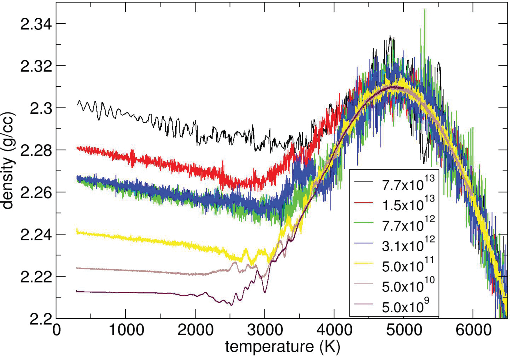
\includegraphics[height=4.6cm]{chapters/chapter6/figures/Lane_density1.pdf}}
    \hfill
    \subfigure[\label{fig:silica-bks-density-temp}]{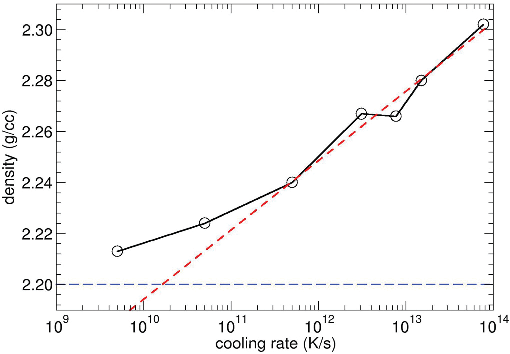
\includegraphics[height=4.6cm]{chapters/chapter6/figures/Lane_density2.pdf}}
    \caption{
    (a) Density vs temperature of a-SiO$_2$, modeled with the BKS potential, for seven quenches completed with linear cooling rates $\gamma$ from $8000\un{K}$ to $300\un{K}$. Silica's density anomaly is visible at high temperatures; density becomes independent of $\gamma$ at $T \gtrsim 4500\un{K}$. 
    (b) Density at $300\un{K}$ as a function of the quench cooling rate $\gamma$. The horizontal dashed line is the experimental value. The red dashed line is a linear extrapolation fit to data above $3\times 10^{12}\un{K/s}$. 
    Reproduced from Ref.~\cite{Lane2015}}
    \label{fig:silica-bks-density}
\end{figure}

The glass transition temperature, that they estimated from the enthalpy curves, increases with $\gamma$. As one can expect, fast cooling rates make the system fall out of equilibrium more quickly during the quench. 
The density $\rho$ of the final sample also depends on the quenching rate: at temperatures below $2000-3000\un{K}$, higher $\gamma$ determine higher densities, as can be observed in Fig.~\ref{fig:silica-bks-density}, that seem to approach the experimental value of $2.202\un{g/cm^3}$. Between $10^{14}\un{K/s}$ and $10^{9}\un{K/s}$ density decreases of less than $5\%$. 
This behaviour is unusual: in most glasses density increases as cooling rates are slowed down. This can be explained by observing the trend at higher temperatures, where the density reaches a maximum at $T\sim 4800\un{K}$ that does not depend on $\gamma$: this ``density anomaly'' is also observed in experiments, at a much lower temperature of $1820\un{K}$. This discrepancy can be attributed to the BKS potential.
%\LEnote{and to the finite size of the simulation domain.}  
Furthermore, the thermal expansion coefficient at constant pressure, $\alpha_p = \frac{1}{V} \left.\frac{\partial V}{\partial T}\right|_p = -\frac{1}{\rho} \left.\frac{\partial \rho}{\partial T}\right|_p$, increases with $\gamma$.

\paragraph{Structural properties}
The structure is even more affected by the quenching rate. 
By analysing the radial distribution function (RDF) between different species it is possible to observe that a small cooling rate makes the structural order at short and intermediate distances increase, \emph{i.e.} the RDF peaks and minima are sharpened and the structure is more relaxed. However, the location of the RDF's peaks is very little affected by $\gamma$ (\emph{i.e.} the Si-O tetrahedra do not change much their size with $\gamma$) and compares quite well with experiment, thus making BKS a good potential to reproduce the short- and medium-range structure of a-SiO$_2$. 
Since the size of Si-O tetrahedra does not change much their size with $\gamma$, the variation of density with the changes in the cooling rate is due to relative arrangement of neighboring tetrahedra. 
This can be observed in variations of the distributions of angles and rings. The O-Si-O angle distribution sharpens by decreasing $\gamma$ and approaches the ideal tetrahedron angle of $109.47^\circ$; the Si-O-Si angle distribution, instead, does not sharpen but shifts to larger angle values, indicating a more open arrangement of tetrahedra, which is consistent with the observed lower density; $6$-vertex rings become more frequent with decreasing $\gamma$, indicating that the local structure of the system approaches the one of $\beta$-crystobalite. 
The study of coordination numbers of each atom type shows that local order increases fast with decreasing cooling rate: for example, the number of Si atoms that are 4-fold coordinated with O atoms increases from $95\%$ to $99.5\%$ by decreasing the cooling rate from $10^{15}\un{K/s}$ to $10^{13}\un{K/s}$, and even further at $10^{10}\un{K/s}$, indicating a gradually decreasing number of coordination defects. 

\paragraph{Vibrational properties}
The two high-frequency peaks of VDOS depend on the quenching rate in that their height increases significantly with decreasing $\gamma$, hence improving the agreement with experiment. 
The low- and mid-frequency bands obtained with the BKS, are quite featureless and do not change very much with $\gamma$, thus remaining quite in discordance with experimental results. 

\medskip
To our knowledge, a study of the dependence of the thermal conductivity of a-SiO$_2$ on the quenching rate has never been performed, and should be completed before attempting a first-principles calculation. In Sec.~\ref{sec:results-class-quench} we will present this study. 

In conclusion, even though these studies have been performed using the BKS potential and not with DFT (for obvious computational reasons), it is very reasonable to assume that their results will also hold for AIMD simulations of amorphous silica. 
The demonstrated capabilities of the BKS potential in structure prediction and the very large range of time scales analysed leads us to conclude that a reliable a-SiO$_2$ structure can only be obtained by a ``slow'' quenching protocol with classical MD. 
AIMD simulations can then be used to optimize the structure, generate a trajectory and, finally, a heat current time series ready to be analysed. 



%%%%%%%%%%%%%%%%%%%%%%%%%%%%%%%%%%%%%%%%%%%%%%%%%%%%%%%%%%
\section{Classical preliminaries}  \label{sec:results-classical}

\subsection{Force field}  \label{sec:results-class-force-field}
\begin{figure}[!tb]
    \centering
    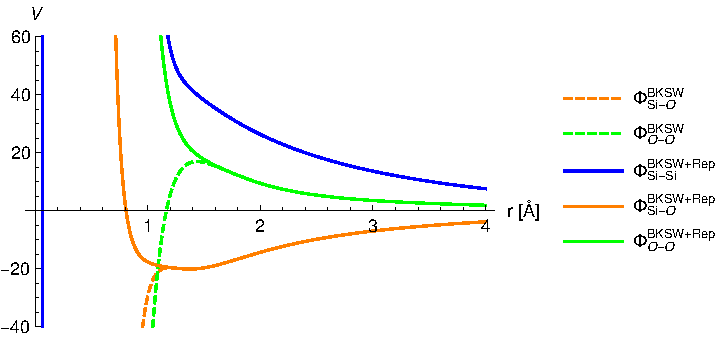
\includegraphics[]{chapters/chapter6/figures/BKSW.pdf}
    \caption{Dashed lines: BKS potential with Wolf truncation, as defined in Eq.~\eqref{eq:BKS-Wolf}. Solid lines: the same with a repulsive core added, defined in Eq.~\eqref{eq:BKS-repulsive-core}.}
    \label{fig:BKS-potential}
\end{figure}

We performed classical MD simulations of amorphous silica using the \textsc{LAMMPS} package \cite{LAMMPS1995}. 
We used a modified version of the BKS potential \cite{Carre2008}, in which the long-range Coulomb interaction is truncated with the Wolf method \cite{Wolf1992,Wolf1999,Fennel2006}, thus avoiding the use of Ewald summations \cite{Allen1989,Frenkel2001}. This truncation is possible thanks to Coulomb screening effects, and it only needs the addition of a correction term that recovers the requirement of charge neutrality. 
The final form we used is the one of Ref.~\cite{Mantisi2012}:
\begin{multline}
    v_{\alpha\beta}^{\mathrm{BKS}}(R) = q_\alpha q_\beta \mathtt{e}^2 V_W(R) G_W(R) + \\
    \left[ A_{\alpha\beta} \mathrm{e}^{-\frac{R}{\rho_{\alpha\beta}}} - \frac{C_{\alpha\beta}}{R^6} - \left( A_{\alpha\beta} \mathrm{e}^{-\frac{R_{c,\mathrm{sh}}}{\rho_{\alpha\beta}}} - \frac{C_{\alpha\beta}}{R_{c,\mathrm{sh}}^6} \right) \right] G_{\mathrm{sh}}(R) , \label{eq:BKS-Wolf}
\end{multline}
with
\begin{equation}
    V_W(R) = \left(\frac{1}{R}-\frac{1}{R_c}\right) + \frac{1}{R_c^2}\left(R-R_c\right) ,
\end{equation}
\begin{equation}
    G_W(R) = \exp \left( -\frac{\gamma_W^2}{(R-R_{c,W})^2} \right) , \quad
    G_{\mathrm{sh}}(R) = \exp \left( -\frac{\gamma_{\mathrm{sh}}^2}{(R-R_{c,\mathrm{sh}})^2} \right) ,
\end{equation}
$q_{\mathrm{Si}}=2.4$, $q_{\mathrm{O}}=-1.2$, $\gamma_W = \gamma_{\mathrm{sh}} = 0.5$, $R_{c,W} = 10.17\un{\angstrom}$, and $R_{c,\mathrm{sh}} = 5.5 \un{\angstrom}$.
This potential, whose form is depicted in Fig.~\ref{fig:BKS-potential}, was shown to give results comparable to the original BKS formula \cite{Carre2008}. 
Since the potential becomes attractive at very short distances, its short-range part at $R < R_{\mathrm{inf}}$ has been substituted by a repulsive core, in order to prevent atoms from getting too close to each other: a problem that may arise at high temperatures during melting. The form of this repulsive part is:
\begin{equation}
    V_{\alpha\beta}^{\mathrm{rep}}(R < R_{\mathrm{inf}}) = \frac{D_{\alpha\beta}}{R^{12}} + E_{\alpha\beta}R + F_{\alpha\beta}, \label{eq:BKS-repulsive-core}
\end{equation}
that we designed such that the potential and its first and second derivatives are continuous, as depicted in Fig.~\ref{fig:BKS-potential}. The parameters of the potential are reported in Table~\ref{tab:BKS-table}. 

\begin{table}[!tb]
    \centering
    \begin{tabular}{c|ccccccc}
        $\alpha$-$\beta$ & $A_{\alpha\beta}\un{(eV)}$ & $\rho_{\alpha\beta}\un{(\angstrom)}$ & $C_{\alpha\beta}\un{(eV\angstrom^6)}$ & $D_{\alpha\beta}\un{(eV\angstrom^{12})}$ \\
        \hline
        O-O   & $1388.773$    & $0.3623$ & $175.0$     & $142.209126863$ \\
        Si-O  & $18003.7572$  & $0.2052$ & $133.5381$  & $1.434274208$ \\
        Si-Si & $872360308.1$ & $0.0657$ & $23.299907$ & $0.0$ \\
        \hline
        \hline
        $\alpha$-$\beta$ & $E_{\alpha\beta}\un{(eV\angstrom^{-1})}$ & $F_{\alpha\beta}\un{(eV)}$ & $r_{\mathrm{inf}}\un{(\angstrom)}$ \\
        \hline
        O-O   & $-14.9704268$ & $39.035745917$  & $1.75$ \\
        Si-O  & $-3.2771769$  & $-15.797166326$ & $1.27$ \\ 
        Si-Si & $0.0$         & $0.0$           & $0.0$
    \end{tabular}
    \caption{Parameters of the BKS potential used in classical MD simulations, defined in Eq.~\eqref{eq:BKS-Wolf} and \eqref{eq:BKS-repulsive-core}.}
    \label{tab:BKS-table}
\end{table}


\paragraph{Simulation protocol}
We started the simulation from a $72$-atom sample of $\beta$-cristobalite, corresponding to $24$ SiO$_2$ units, that we eventually replicated to obtain larger cubic supercells at the experimental density of a-SiO$_2$, $\rho = 2.202\un{g/cm^3}$. 
Each system was melted and equilibrated at constant temperature $7000\un{K}$ for more than $t_{\mathrm{melt}} = 500\un{ps}$ in the NVT ensemble, using the Bussi-Donadio-Parrinello stochastic velocity-rescaling thermostat \cite{Bussi:2007cs} with a coupling time constant $\tau_\mathrm{NVT}=200\un{fs}$. The equations of motion were integrated using the velocity Verlet algorithm with a time step of $\epsilon_\mathrm{MD}=1\un{fs}$. 
Subsequently, the temperature was decreased linearly in a time $t_{\mathrm{quench}}$ down to $T_{\mathrm{eq}}=500\un{K}$, in the NVT ensemble, thus resulting in a quenching rate of $\gamma = \frac{6500\un{K}}{t_{\mathrm{quench}}}$. The effects of different quenching rates will be studied in Sec.~\ref{sec:results-class-quench}. 
The system was equilibrated at $T_{\mathrm{eq}}$ in the NVT ensemble for other $400\un{ps}$, and finally in the microcanonical (NVE) ensemble for $100\un{ps}$. 
At this point, we started to collect data for at least $t_{\mathrm{run}} = 1\un{ns}$. 

The computational cost of these classical simulations is very low, so it was possible to run different replicas of each system from different initial conditions, thus providing us with abundant statistics. 
The thermal conductivity was estimated from $t_{\mathrm{run}} = 1\un{ns}$ of trajectory for each sample, using the \emph{cepstral analysis} method presented in Sec.~\ref{sec:cepstral-analysis}.

%\begin{itemize}
%    \item NVT:  300 (deform) + 200(NVT) + 500(NVT)            + ramp + 400(NVT) + 100(NVE)
%    \item NPT:  300 (deform) + 100(NPT) + 300(NVT) + 100(NPT) + ramp + 200(NPT) + 200(NVT) + 100(NVE)
%\end{itemize}


\subsection{Sample preparation: size and quenching rate dependence of \texorpdfstring{$\kappa$}{thermal conductivity}}  \label{sec:results-class-quench}
In order to study the convergence of lattice thermal conductivity with the size of the system and the quenching rate, we considered cells containing $72$, $144$, $288$, $432$, $576$, $864$, $1152$, $2304$, $5184$, and $10800$ atoms. For each cell size we analysed the data obtained from $10$ independent replicas with different initial conditions. 
For each replica, we considered $10$ different quenching times: $t_{\mathrm{quench}} = 5$, $10$, $25$, $50$, $100$, $250$, $500\un{ps}$, $1$, $5$, and $10\un{ns}$, that correspond to quenching rates $\gamma$ ranging from $1.3\times 10^{15}$ to $6.5\times 10^{11}\un{K/s}$.
We computed the thermal conductivity $\kappa$ of each of these samples, from a trajectory of $t_\mathrm{run}=1\un{ns}$, using \emph{cepstral analysis}. More technical details on this procedures are reported in Sec.~\ref{sec:cepstral-analysis}. 

\begin{figure}[!tb]
    \centering
    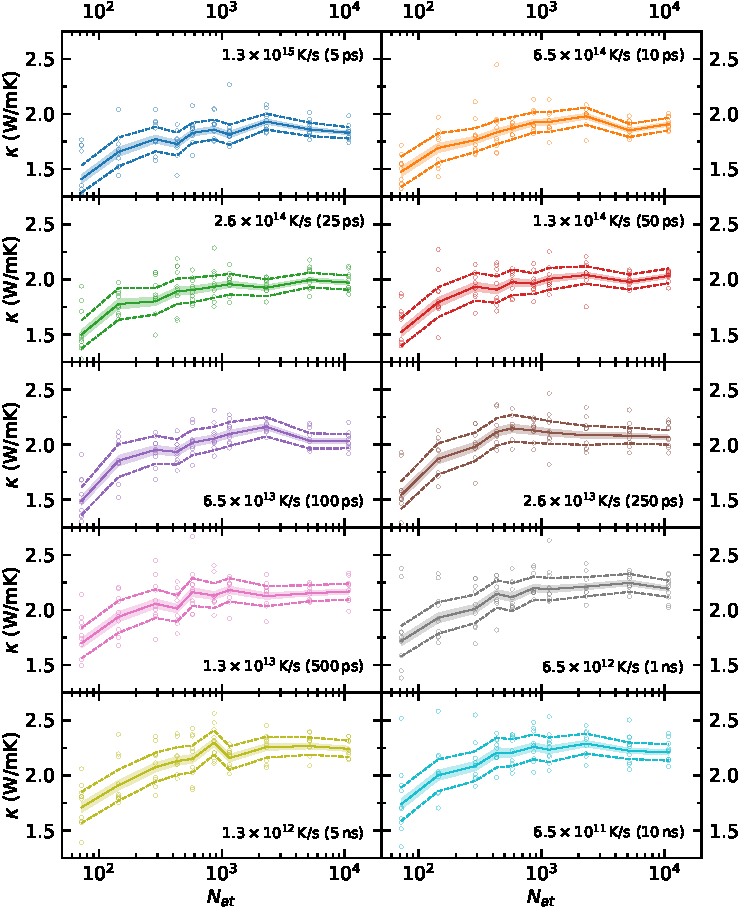
\includegraphics[width=\textwidth]{chapters/chapter6/figures/Silica_NVT_kappa_NATconv_tesi.pdf}
    \caption{Study of convergence of the thermal conductivity of a-SiO$_2$ at $500\un{K}$ with the size of the system, estimated from classical simulations, as described in Sec.~\ref{sec:results-class-quench}. 
    The abscissa indicates the number of atoms of the system, each panel corresponds to a different quenching rate $\gamma$ (the relative quenching time $t_\mathrm{quench}$ is indicated in brackets). 
    Circles are the results of $10$ independent replicas simulated with the same quenching protocol. The solid line is a weighted average computed over the replicas and weighted using the errors estimated from cepstral analysis. Three different error limits are indicated. 
    Dashed area: standard deviation of the weighted mean. 
    Dashed lines: statistical error estimated for a \emph{single} $1\un{ns}$-trajectory. 
    %\LEcancel{Dotted lines: sample standard deviation of the single values of $\kappa$.}\LEnote{**RIMUOVERE LINEE PUNTINI**}
    }
    \label{fig:results-class-kappa-vs-size}
\end{figure}

In Fig.~\ref{fig:results-class-kappa-vs-size} we plot the thermal conductivity as a function of the number of atoms of the system $N_{at}$, for the ten quenching rates considered. 
The $\kappa$ measured for each replica is depicted with a circle. 
For each $N_{at}$ and $\gamma$, we computed a weighted average over the replicas' results (depicted with a solid line) using the errors estimated from cepstral analysis as weights. 
We can infer that $\kappa$ is underestimated by the smallest systems considered, and seems to converge to a stable value for $N_{at}\gtrsim 500$ atoms. 
This is likely due to two effects, both entering this analysis. 
The first is the fact that small replicas cannot account for the whole ensemble of possible amorphous structures. In particular, the variety of medium- and long-range structures needs larger system to be correctly accounted for. However, as we mentioned in Sec.~\ref{sec:silica-size}, some authors found that averaging over a little set of small structures ($N_{at}=72$) should be enough to reproduce fairly well the range of glass-network structures found in larger cells \cite{VanGinhoven2005}. 
Nevertheless, the smallest systems lead to an underestimate of $\kappa$ by more than $20\%$. We can probably attribute this behaviour to a second effect, affecting the vibrational modes: the finite-size of the system dictates an upper limit to the wavelength that can be accommodated into the simulation cell, and alters the the low and medium vibrational frequencies, which are largely attributed to the collective modes of silica. The Green-Kubo equation thus requires a sufficiently large volume to correctly account for all the contributions. 
We should however point out that this value is remarkably lower (approximately ten times lower) than the typical cell volumes required by NEMD calculations.

\begin{figure}[!tb]
    \centering
    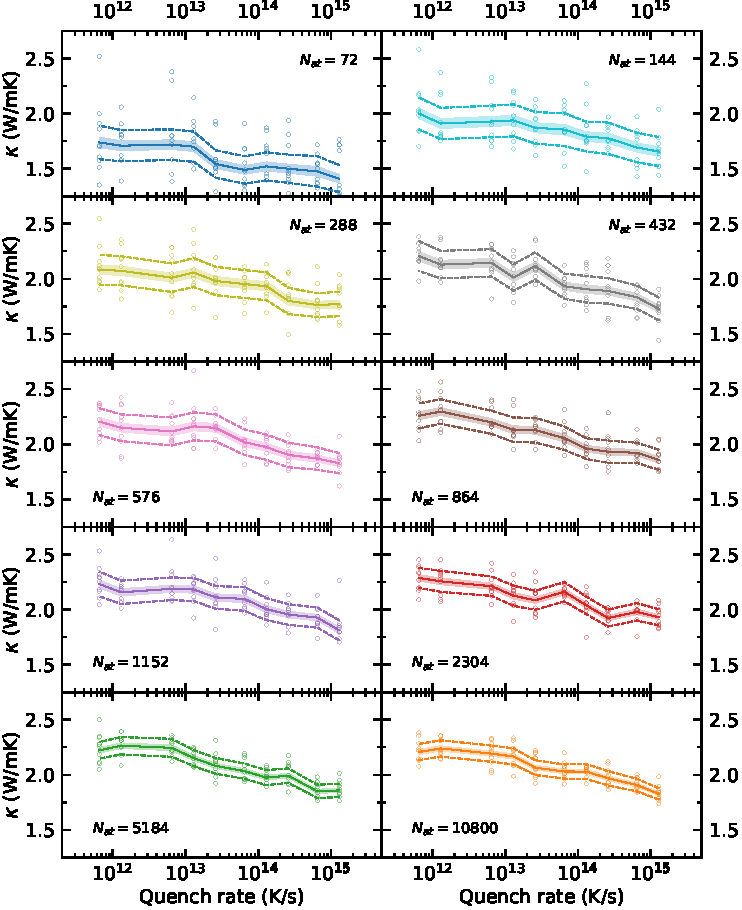
\includegraphics[width=\textwidth]{chapters/chapter6/figures/Silica_NVT_kappa_QTIMEconv_tesi.pdf}
    \caption{Study of convergence of the thermal conductivity of a-SiO$_2$ at $500\un{K}$ with the cooling quenching rate $\gamma$, estimated from classical simulations, as described in Sec.~\ref{sec:results-class-quench}. 
    Each panel corresponds to a different system size with $N_{at}$ atoms.
    Circles are the results of $10$ independent replicas simulated with the same quenching protocol. The solid line is a weighted average computed over the replicas and weighted using the errors estimated from cepstral analysis. Three different error limits are indicated. 
    Dashed area: standard deviation of the weighted mean. 
    Dashed lines: statistical error estimated for a \emph{single} trajectory of $1\un{ns}$. 
    %\LEcancel{Dotted lines: sample standard deviation of the single values of $\kappa$.}\LEnote{**RIMUOVERE LINEE PUNTINI**}
    }
    \label{fig:results-class-kappa-vs-quench}
\end{figure}

In Fig.~\ref{fig:results-class-kappa-vs-quench}, the same data are plotted as a function of the quenching rate $\gamma = \frac{6500\un{K}}{t_{\mathrm{quench}}}$, for each of the sizes considered. 
Slower quenching rates (longer quenching times, of the order of a few nanoseconds) definitely lead to higher thermal conductivities. 
This is not very surprising: as we discussed in Sec.~\ref{sec:silica-quenching}, a slower quenching allows the system to relax more and to build glass structures with higher local order, less defects, and structural features that are in better agreement with experiments. 
Therefore, a quenching rate $\gamma \lesssim 10^{13}\un{K/s}$ seems to be the requirement for almost all the simulated sizes. 

In Fig.~\ref{fig:results-class-kappa-vs-size} and \ref{fig:results-class-kappa-vs-quench} the error on the weighted average is indicated as a thin shaded area surrounding the solid line. Two other lines are reported. The dashed lines delimit the average error that we expect to obtain from a single trajectory sample of $t_{\mathrm{run}}=1\un{ns}$ (it is about the error on the weighted averaged times $\sqrt{10}$). 
We observe that in general the single calculations of $\kappa$ ($10$ replicas for each abscissa, represented by single circles), fall mostly inside this error bars, for the medium and large systems. For the smaller systems, the fluctuations of the single values become larger, probably due to larger differences in their structures, in addition to the intrinsically larger fluctuations due to the smaller size. 
%\LEcancel{The fluctuations of $\kappa$ can also be quantified by the standard deviation of $\kappa$ computed over the replicas, indicated with thin dotted lines, that becomes visibly larger than the expected error bars for the two or three smallest systems analyzed (even though this value, estimated from a very small sample, should be taken as indicative).}
The trend of the relative error estimated for a $1\un{ns}$ trajectory as a function of the number of atoms is shown in Fig.~\ref{fig:results-class-kappaerror-vs-size}, for $4$ selected quenching rates, and seems to decrease as $\sim 1/\sqrt{N_\mathrm{nat}}$. 
The quenching rate, instead, does not appear to affect the error on $\kappa$, as shown in Fig.~\ref{fig:results-class-kappaerror-vs-quench}. 

\begin{figure}[!tb]
    \centering
    \subfigure[\label{fig:results-class-kappaerror-vs-size}]{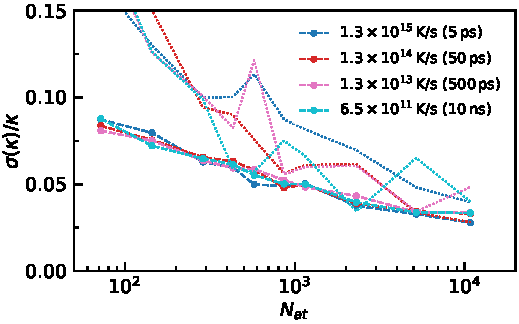
\includegraphics[width=0.49\textwidth]{chapters/chapter6/figures/silica_NVT_kappa_relerror_NAT.pdf}}
    \hfill
    \subfigure[\label{fig:results-class-kappaerror-vs-quench}]{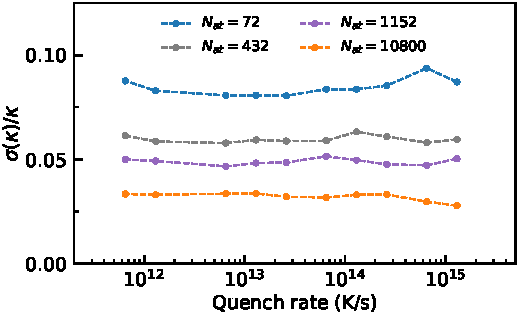
\includegraphics[width=0.49\textwidth]{chapters/chapter6/figures/silica_NVT_kappa_relerror_QTIME.pdf}}
    \caption{Estimated relative error on the thermal conductivity of a-SiO$_2$ for a $1\un{ns}$ trajectory (dashed lines) as a function of (a) the number of atoms, (b) the cooling quenching rate. 
    %\LEcancel{Dotted lines: sample standard deviation of the single values of $\kappa$.}\LEnote{**RIMUOVERE LINEE PUNTINI**}
    }
    \label{fig:results-class-kappaerror}
\end{figure}

From this analysis we conclude that system size and cooling rate considerably affect the thermal conductivity of BKS silica glass. 
In order to perform an \abinitio study of the thermal conductivity, we need to select a sample size that can be simulated with AIMD at a reasonable computational cost. 
We decided to use one of the samples with $N_{\mathrm{at}}=432$ atoms that were generated using the smallest cooling rate analysed, $\gamma=6.5\times 10^{11}\un{K/s}$, corresponding to a quenching time of $10\un{ns}$. In the following we dub this sample $\S1$. 
We first made sure that $\S1$ did not exhibit any coordination defects, then we computed its thermal conductivity, that results to be $\kappa_\S1 = (2.207 \pm 0.045) \un{W/mK}$, using a $1\un{ns}$-long trajectory. 
This value differs from the average values obtained for the largest systems analyzed by less than $5\%$ ($\approx 0.1\un{W/mK})$. 
Further data analysis showed that an error of the order of $12\%$ ($\approx 0.25\un{W/mK}$) could be obtained from a trajectory of $100\un{ps}$, a simulation length reasonably affordable with CPMD, hence making this bias in the thermal conductivity negligible. 



\subsection{Cepstral analysis}  \label{sec:results-class-cepstral}
The thermal conductivity of each classical replica of silica was computed with the cepstral analysis technique described in Sec.~\ref{sec:cepstral-analysis}. 
The $P^*$ cutoff was chosen using the Akaike Information Criterion (see Sec.~\ref{sec:AIC}) without any correction factor, because in Sec.~\ref{sec:cepstral-benchmarks} we showed that this was not necessary for the case of classical a-SiO$_2$. 
The heat flux calculated by \textsc{LAMMPS} at each time step ($1\un{fs}$) was filtered with a moving average and resampled at a rate of one step every $18\un{fs}$, corresponding to a cutoff frequency $f^*\approx 28\un{THz}$. The resulting spectrum was analyzed using our \textsc{ThermoCesptrum} code \cite{thermocepstrum}.
In the following we perform an additional analysis on the dependence of the thermal conductivity of the $\S1$ sample on some of the parameters. 

\begin{figure}[!tb]
    \centering
    \subfigure[\label{fig:csilica-sample-expdens-fstar-100ps}]{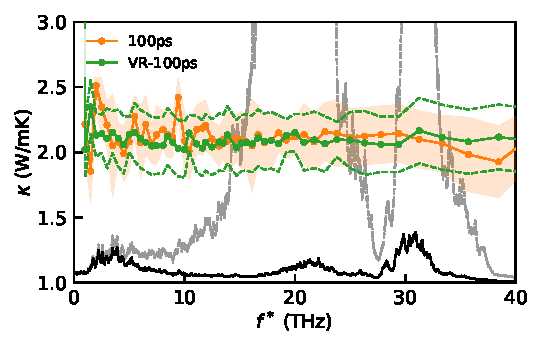
\includegraphics[width=0.49\textwidth]{chapters/chapter6/figures/silica_expdens_kappa_fstar_VR_100ps.pdf}}
    \hfill
    \subfigure[\label{fig:csilica-sample-expdens-fstar-1ns}]{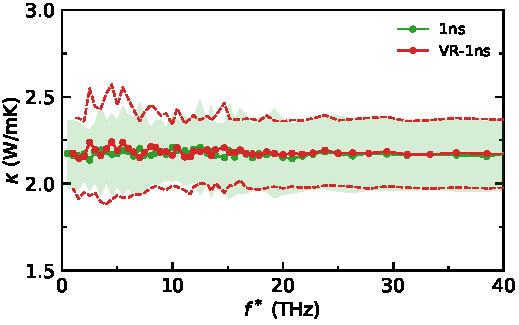
\includegraphics[width=0.49\textwidth]{chapters/chapter6/figures/silica_expdens_kappa_fstar_VR_1ns.pdf}} \\
    \subfigure[\label{fig:csilica-sample-expdens-fstar-10ns}]{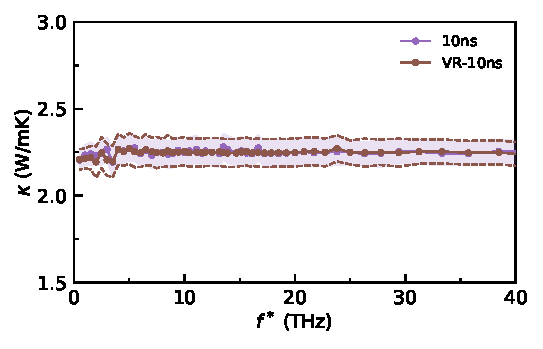
\includegraphics[width=0.49\textwidth]{chapters/chapter6/figures/silica_expdens_kappa_fstar_VR_10ns.pdf}}
    \hfill
    \subfigure[\label{fig:csilica-sample-expdens-psd-VR}]{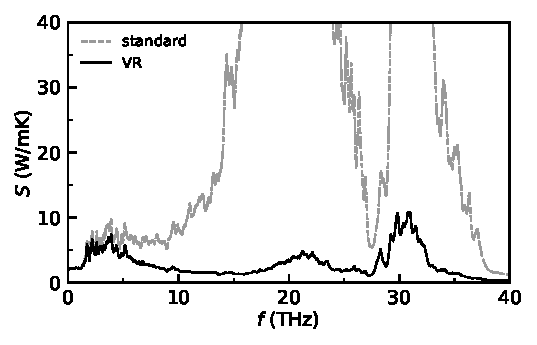
\includegraphics[width=0.49\textwidth]{chapters/chapter6/figures/silica_expdens_psd_VR_10ns.pdf}}
    \caption{Dependence of $\kappa$ on the choice of the cutoff frequency $f^*$, estimated from \emph{one} sample of (a) $100\un{ps}$, (b) $1\un{ns}$, and (c) $10\un{ps}$ of the ``original'' and VR heat flux time series; (d) periodograms of the original and the VR heat flux time series.}
    \label{fig:csilica-sample-expdens-fstar}
\end{figure}

We first study the value of the thermal conductivity estimator as a function of the cutoff frequency $f^*$ and the length of the trajectory. 
In Fig.~\ref{fig:csilica-sample-expdens-fstar}(a-c) we report the average $\kappa$ obtained for a $100\un{ps}$, $1\un{ns}$, and $10\un{ns}$ trajectory, respectively. 
In general, all the $f^*$ in the middle region give compatible results, with more instabilities arising at the lowest frequency values (likely due to increasing aliasing effects that alter the spectrum), that indeed show an increased error and and should be avoided in this case. These fluctuations decrease in longer trajectories, as the statistical error obviously decreases. Besides, a too high $f^*$ ($f^*\gtrsim 60\un{THz}$, not shown) induces a bias in $\kappa$, due to the fact the log-periodogram diverges to negative values and we start to have problems of numerical accuracy. 
A $100\un{ps}$ trajectory ultimately gives compatible results with the $10\un{ns}$ one, as reported in Table~\ref{tab:csilica-sample-kappa-cepstral}
Incidentally, we also notice that the error on $\kappa$ estimated by cepstral analysis decays slower than expected with the length of the trajectory. Indeed the error should decrease as the inverse of the trajectory length (see Eq.~\eqref{eq:sigma*}), but from $100\un{ps}$ to $1\un{ns}$ it decreases of a factor $\approx \frac{1}{\sqrt{3}}$, and a factor $\approx \frac{1}{\sqrt{10}}$ from $100\un{ps}$ to $10\un{ns}$. This effect can be explained by the increased number of cepstral coefficients retained by the AIC, that tries to reproduce the finest features of the spectrum with greater precision. 

\begin{table}[!tb]
    \centering
    \begin{tabular}{r|cc|c}
        $t_\mathrm{run}$ & \textbf{standard-HC} & \textbf{VR-HC} & \textbf{$\langle P^* \rangle$} \\
        \hline
        $100\un{ps}$ & $2.19 \pm 0.25\: (12\%)$  & $2.17 \pm 0.27\: (12\%)$ & $47-36$\\
        $1\un{ns}$   & $2.18 \pm 0.15\: (9.5\%)$ & $2.18 \pm 0.20\: (9.2\%)$ & $176-154$ \\
        $10\un{ns}$  & $2.24 \pm 0.08\: (3.5\%)$ & $2.25 \pm 0.07\: (3.3\%)$ & $448-377$
    \end{tabular}
    \caption{Estimated statistical error on the thermal conductivity of sample $\S1$ for a trajectory length $t_\mathrm{run}$. ``Standard-HC`` and ``VR-HC'' refer to the standard definition of the heat current and the equivalent definition with renormalized atomic velocities, respectively. The last column contains the average number of cepstral coefficients retained using the standard and VR heat current, respectively. }
    \label{tab:csilica-sample-kappa-cepstral}
\end{table}

We also analyzed a ``decorrelated'' heat current, obtained by the velocity-renormalization (VR) method described in Sec.~\ref{sec:gauge-renormalization}. As shown in Fig.~\ref{fig:csilica-sample-expdens-psd-VR}, this method reduces the power of the spectrum by a large amount, removing part of the signal at finite frequencies that does not contribute to the thermal conductivity, without affecting the low-frequency region, hence the value at zero frequency. 
This procedure is very useful to reduce the variance of the energy current signal obtained from \abinitio simulations, however here it does not change much the results, nor the statistical error in a significant way, as reported in Table~\ref{tab:csilica-sample-kappa-cepstral}. 
The number of cepstral coefficients $P^*$ is reduced as the spectrum is smoother, but the error ultimately increases if we use a low $f^*$ , due to the fact that the optimal $P^*$ becomes too low. 



\subsection{Density dependence of \texorpdfstring{$\kappa$}{thermal conductivity}}
The dependence of $\kappa$ of a-SiO$_2$ on the pressure can be safely neglected for the range of temperatures considered later ($300-1500\un{K}$). 
Silica glass has a anomalously low thermal expansion coefficient, with an experimental value of $\alpha = \frac{1}{V}\left(\frac{\partial V}{\partial T}\right)_T \approx 5.5\times 10^{-7} \un{K^{-1}}$ at $300\un{K}$, about $20$ times smaller than that of crystalline forms of silica. 
The relative variation in density from $300\un{K}$ to $1500\un{K}$ can be estimated to be $\frac{\Delta\rho}{\rho} \approx 7\times 10^{-4}$.
Using the experimental bulk modulus $K=-V\frac{dP}{dV}=\rho\frac{dP}{d\rho}\approx 36.7\un{GPa}$ and experimental density at $300\un{K}$, $\rho=2.202\un{g/cm^3}$, we can expect a consequent variation in pressure of about $\Delta P \approx 30\un{MPa}$, quite negligible. 
Experimental measures of thermal conductivity of silica at high pressures estimate a variation of $\kappa$ with pressure of the order of $5\%/\mathrm{GPa}$ \cite{Andersson1992}, hence we can safely neglect this effect. 

In classical simulations these values may change slightly, but we do not expect significant differences. 
In the preliminary phases of this work we also performed quenching simulations at constant pressure, in the NPT ensemble. 
We found, in accordance with previous studies discussed in Sec.~\ref{sec:silica-quenching}, that the density of the sample increases with the quenching rate. A slow quenching leads to lower densities, closer to the experiment. The average equilibrium density obtained from the slowest quench at zero pressure is equal to $\rho_{P=0}=2.31\un{g/cm^3}$, slightly larger than the experimental one. We can attribute this discrepancy to a combined effect of the BKS potential and of the fast quenching rate. 
The thermal expansion coefficient is $5$ times larger than experiment, with a value of $\alpha\approx 2.8\times 10^{-6} \un{K^{-1}}$. 
Finally, the thermal conductivities obtained from quenches in the NPT ensemble show values that are up to $10\%$ larger than those obtained by quenches at fixed volume, for the fastest quenching rates and smallest sizes, and of similar values for the slowest rates (plots obtained from the NPT simulations are reported in Appendix~\ref{ch:appendix-npt-results}). 
The slightly higher densities (up to $\approx 2.5\un{g/cm^3}$) that are obtained by using very fast quenching rates are probably the reason of this difference. 
We decide therefore to set the density at the experimental value and to equilibrate our simulations in the NVT ensemble, as previously done by many authors.
%\LEnote{Grafici $\rho(\gamma)$ e $\kappa(\rho)$ in appendice}


%%%%%%%%%%%%%%%%%%%%%%%%%%%%%%%%%%%%%%%%%%%%%%%%%%%%%%%%%%%%5
\section{Quantum simulations: results}  \label{sec:results-quantum}
The $\S1$ sample has been simulated with Car-Parrinello MD using the \texttt{cp.x} code of the \textsc{Quantum ESPRESSO} suite \cite{Giannozzi2009,Giannozzi2017}. 
We used the PBE-GGA exchange-correlation functional \cite{Perdew1996}, wave functions were expanded in plane waves with a kinetic-energy cutoff of $70\un{Ry}$ and using the optimized norm-conserving Vanderbilt pseudopotentials (ONCVP) \cite{Schlipf2015,Hamann2013}. The cutoff was chosen so that energies and forces were converged.
The system contained $432$ atoms ($144\,$Si, $288\,$O) and $2304$ electrons. A time step of $\epsilon_\textrm{CP} = 15\un{a.u.} \approx 0.36\un{fs}$ and a fictitious electron mass of $400\un{a.u.}$ were used to integrate the equations of motion. 
We verified that the kinetic energy of the fictitious electronic degrees of freedom and the total energies were not drifting during the whole length of the simulation. 
The system was thermalised for about $5\un{ps}$ at temperature $T_\mathrm{eq}$ in the NVT ensemble using the Nos\'e-Hoover thermostat \cite{Nose1984,Hoover1985}, then it was let evolved in the microcanonical ensemble for about $t_\mathrm{run}\approx 52\un{ps}$. 
No atomic diffusion or significant structural modifications were observed during the whole \abinitio MD runs.

Four different equilibrium temperatures $T_\mathrm{eq}$ were simulated: $300$, $500$, $1000$, and $1500\un{K}$. For each temperature we actually ran two independent simultaneous simulations with different initial conditions, thus obtaining a total of $\approx 105\un{ps}$ worth of data at each temperature, in half the wall time. 
Each of the CPMD calculations costed about $140\un{k}$ CPU hours.

%\LE{**tabella dati??*}


\subsection{Heat current calculation}  \label{sec:results-quantum-current}
For each AIMD trajectory generated, we proceeded to the computation of the \abinitio heat current, following the procedure described in Sec.~\ref{sec:dft-hc-computation}. 
The first important parameter to fix is the heat current sampling rate. For this system, we estimated that one single-step calculation of the current costs roughly $60$ CPU hours, so one can easily estimate the potential cost of a $100\un{ps}$ trajectory. 


\paragraph{Heat current sampling rate}
In fact, the time period $\epsilon_\mathrm{HC}$ over which we compute the current determines the Nyqvist frequency of its power spectrum, $f_\mathrm{Ny}$, \emph{i.e.} the maximum frequency reproducible (see Sec.~\ref{sec:cepstral-nyqvist}), therefore we have to make sure that the maximum frequency of the power spectrum is smaller than $f_\mathrm{Ny}$. Of course, the longer $\epsilon_\mathrm{HC}$, the smaller the number of steps we will need to compute. 
An educated guess can be made from classical MD simulations. By examining the power spectrum of the classical heat current, we estimated that a sampling period $\epsilon_\mathrm{HC} = 30 \epsilon_\mathrm{CP} \approx 10.88\un{fs}$ would give a reasonably low $f_\mathrm{Ny}\approx 45\un{THz}$. 
If we resample the classical time series at different sampling rates, without applying any preliminary filter, we observe the effects of aliasing on the power spectrum. 
After some trials, we verified that sampling rates leading to a decrease of spectral power $\Delta\mathsf{P}$ (the integral of the power spectrum) of less than $1\%$ do not appreciably introduce aliasing effects that may alter the low-frequencies of the spectrum, hence the value of thermal conductivity. A value $f_\mathrm{Ny} \approx 40\un{THz}$ ($\Delta\mathsf{P} \approx 0.9\%$) does not change the estimated $\kappa$; choosing $f_\mathrm{Ny} \approx 35\un{THz}$, instead, cuts a tail of the spectrum ($\Delta\mathsf{P} \approx 4\%$) and introduces important aliasing effects that ultimately change its value at zero-frequency, so it should not be used. 

Notwithstanding these considerations, past experience with other systems suggests us that the \abinitio heat current often possess a larger variance than the classical one, (see Sec.~\ref{sec:gauge-renormalization}) hence a larger spectral power, that may invalidate the empirical tests just performed. 
To verify that this was not the case, we decided to compute the \abinitio heat current of a short trajectory at every $20$ CP time steps ($\epsilon_\mathrm{HC} = 20 \epsilon_\mathrm{CP} \approx 7.26\un{fs}$), and compare the results obtainable from different sampling periods: $\epsilon_\mathrm{HC} = 20\epsilon_\mathrm{CP}$, $30\epsilon_\mathrm{CP}$, $40\epsilon_\mathrm{CP}$, and $60\epsilon_\mathrm{CP}$. 
The corresponding periodograms are plotted in Fig.~\ref{fig:results-quantum-dt-choice}. The two largest sampling periods, $40\epsilon_\mathrm{CP}$ and $60\epsilon_\mathrm{CP}$, clearly display remarkable aliasing effects, that affect the low- and middle-frequency region of the spectrum, an effect not present if we choose $30\epsilon_\mathrm{CP}$. 
Therefore, we decided to set $\epsilon_\mathrm{HC} = 30\epsilon_\mathrm{CP}$. For a trajectory of $100\un{ps}$, we need to perform about $9500$ heat current calculations, with a total estimated cost of the order of $560\un{k}$ CPU hours. 

\begin{figure}[!tb]
    \centering
    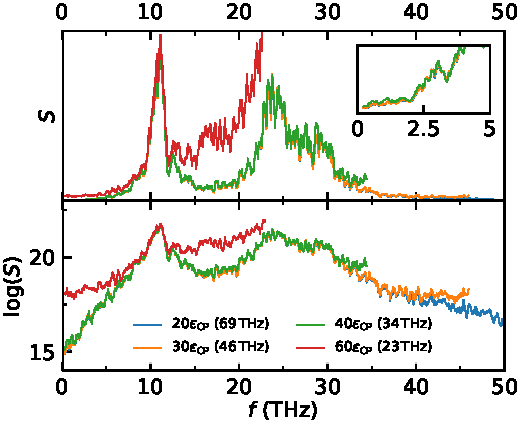
\includegraphics[width=10cm]{chapters/chapter6/figures/qsilica_432_1500K_dt_choice.pdf}
    \caption{Power spectral density of the \abinitio heat current of sample $\S1$ (upper panel) and its logarithm (lower panel), computed from a short trajectory at $1500\un{K}$ at different sampling periods (the resulting $f_\mathrm{Ny}$ are reported in parenthesis). Inset: zoom of the low-frequency region of the spectrum.}
    \label{fig:results-quantum-dt-choice}
\end{figure}


\paragraph{Heat current power spectrum}
\begin{figure}[!tb]
    \centering
    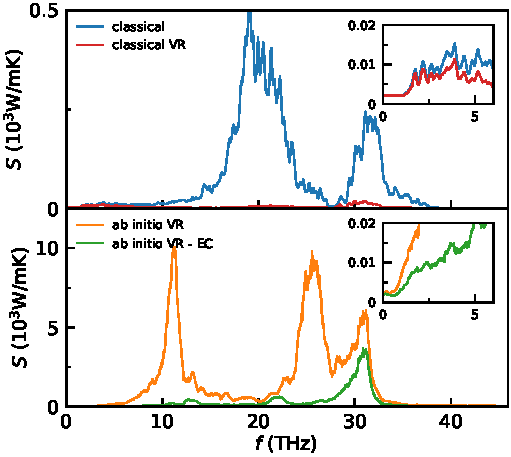
\includegraphics[width=10cm]{chapters/chapter6/figures/silica_cl-q_psd_cfr.pdf}
    \caption{Power spectral density of the heat current of $\S1$ at $300\un{K}$. Upper panel: classical current (blue) and the same with renormalized velocities. Lower panel: \abinitio current with renormalized velocities (orange) and the same decorrelated from the electronic current (green).}
    \label{fig:results-quantum-psd-cfr}
\end{figure}

As we just mentioned, the \abinitio heat current time series has a variance much larger than the classical one, thus making the peaks of its power spectrum much higher, and its analysis possibly more difficult. 
This effect is due to the different definition of the microscopic energy density in the classical and DFT approach, and its different ripartition between atoms. 
Similarly to what happens in a molecular system like water (see Sec.~\ref{sec:MolecularFluids}), the average distance between atoms in a solid is a bounded vector if atomic diffusion does not occur, so we can expect a flux $\mathbf{J}^\mathrm{SiO}=\mathbf{J}^\mathrm{Si}-\mathbf{J}^\mathrm{O}$, where $\mathbf{J}^\mathrm{Si}$ and $\mathbf{J}^\mathrm{O}$ are the number fluxes defined in Eq.~\eqref{eq:JX}, to be a total time derivative of a bounded vector field. By the gauge invariance theorem, we conclude that this flux does not contribute to the thermal conductivity and can therefore be removed with one of the techniques presented in Sec.~\ref{sec:gauge-renormalization}. 

We decided to apply the velocity-renormalization (VR) decorrelation technique before computing the heat current: the value of each atom's velocity (extracted from the CPMD trajectory) was renormalized by subtracting the velocity of the center of mass of its species from it. 
For example, at each time $t$ the velocity of a silicon atom $\mathbf{V}_n(t)$ was substituted with $\mathbf{V}_n(t)-\frac{1}{N_\mathrm{Si}}\sum_{m\in \mathrm{Si}}\mathbf{V}_m(t)$, where $N_\mathrm{Si}$ is the total number of silicon atoms. 
Furthermore, as discussed in Sec.~\ref{sec:dft-electronic-curr}, the electronic current (EC) $\mathbf{J}^{el}$ is also non-diffusive and can therefore be removed, for example by a simple decorrelation procedure applied after the heat current computation. 

The power spectra of the classical and the \abinitio heat currents are displayed in Fig.~\ref{fig:results-quantum-psd-cfr}. One can immediately notice the large difference in power of the classical and \abinitio spectra (see units), and the effects of the VR and EC-decorrelation, that make the spectrum flatter. This effect does not change much the low-frequency region, in the classical case, but it does in the quantum case, even though the convergence at zero-frequency is maintained. 
We also notice that the positions of the peaks of the \abinitio power spectrum are shifted with respect to the classical case, a consequence of the different VDOS of these two systems. 



\subsection{Temperature dependence of \texorpdfstring{$\kappa$}{thermal conductivity}} \label{sec:results-quantum-results}
We now study the thermal conductivity of silica as a function of the temperature and compare it with experimental data.

\paragraph{Experimental data}
\begin{figure}
    \centering
    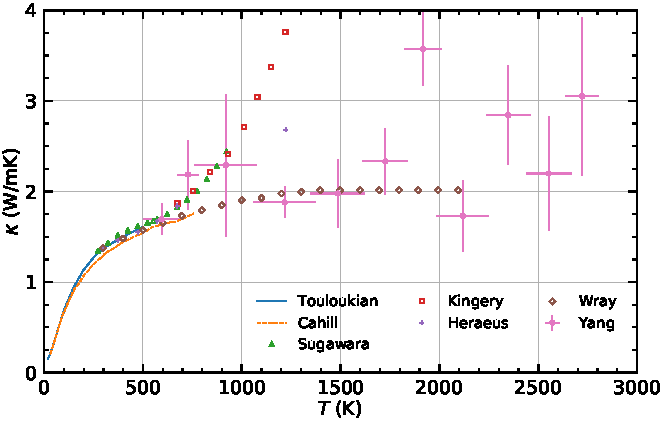
\includegraphics[width=\textwidth]{chapters/chapter6/figures/silica_expkappa.pdf}
    \caption{Experimental measurements of the thermal conductivity of a-SiO$_2$ as a function of the temperature. Data from \citet{Touloukian1970}, \citet{Cahill1990}, \citet{Sugawara1969}, \citet{Kingery1955}, \citet{Wray1959}, \citet{Yang2009}, and data from a glass manufacturer \cite{Heraeus2010}. 
    }
    \label{fig:silica-exp-kappa}
\end{figure}
The first experimental measurements of the thermal conductivity of a-SiO$_2$ as a function of temperature were carried out between the 50's and 70's by \citet{Kingery1955}, \citet{Wray1959}, \citet{Sugawara1969}, and \citet{Touloukian1970}; a few more recent studies are the ones of \citet{Cahill1990} and \citet{Yang2009}. 
We display all these experimental results in Fig.~\ref{fig:silica-exp-kappa}, which shows substantial agreement between all of them at low temperatures, but two different trends at temperatures larger than $600\un{K}$. 
Above $600\un{K}$ radiative heat transport becomes very intense (scaling roughly as $\sim T^{3\div 4}$) and can alter the measured value of $\kappa$, that can be overestimated. This problem is of special importance in vitreous silica because this substance is highly transparent \cite{Carwile1966, Cahill1990, Gardon1961}. \citet{Cahill1990} and \citet{Wray1959} accounted empirically for the radiative effects, thus resulting in a $\kappa$ approaching the value $\kappa\approx 2\un{K/mK}$ for temperatures up to $2000\un{K}$. The recent measures of \citet{Yang2009} performed with CO$_2$ laser heating, instead, did not appear to feature significant radiative contributions. 
Nevertheless, the matter is still under active debate \cite{Bouchut2004}, so at this time no clear experimental values of $\kappa$ are available in this regime. This state of affairs motivates even more an accurate atomistic study to determine the thermal conductivity of a-SiO$_2$ at high temperatures. 

\paragraph{Computational results}
\begin{figure}[!tb]
    \centering
    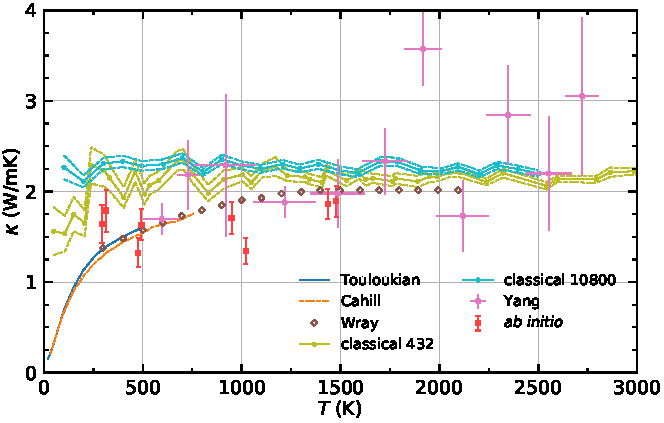
\includegraphics[width=\textwidth]{chapters/chapter6/figures/silica_expkappa_qkappa.pdf}
    \caption{Thermal conductivity of a-SiO$_2$ as function of temperature: comparison between experiments and simulations. 
    Only the experimental studies that accounted for radiative heat transport have been reported. 
    Classical simulations were carried out using the BKS potential for the $\S1$ sample ($432$ atoms), and a larger sample ($10800$ atoms).
    \emph{Ab initio} results were computed using the $\S1$ sample, as described in Sec.~\ref{sec:results-quantum}, by analysing the VR-EC decorrelated energy flux. 
    \LEnote{CHANGE IN classical (432), ab initio (432), AND CHANGE LABEL ORDER}
    }
    \label{fig:results-quantum-kappa-temp}
\end{figure}
In Fig.~\ref{fig:results-quantum-kappa-temp} we display the results of our \abinitio thermal conductivity simulations, compared with the results of classical simulations for the same $432$-atoms sample $\S1$ and a larger sample with $10800$ atoms, and with experimental data. 

The \abinitio thermal conductivities for the eight independent simulations were obtained by analysing the VR-EC decorrelated energy fluxes, with $f^*=f_\mathrm{Ny}$. 
No preliminary filtering and resampling were performed on the time series before cepstral analysis, because the estimated thermal conductivity manifested unusual oscillations by its choice. We attribute this difficulty to two possible causes. 
The first is the relatively large spectral power of the \abinitio energy flux, compared to the classical one, that makes the spectrum raise very quickly at low-frequencies. 
The second and likely most important is ascribable to the small Nyqvist frequency of the \abinitio spectra. Even if no sampling (aliasing) errors are present, as verified in Sec.~\ref{sec:results-quantum-current}, it is likely that the filtering-resampling procedure performed in these conditions will introduce much more spurious (aliasing) effects than it would do for larger $f_\mathrm{Ny}$. 
It is possible that the employment of a different type of low-pass filter would attenuate these side effects. 
Additional in-depth studies on this matter should be performed in the future. 

Nevertheless, the values obtained seem in fairly good agreement with the available experimental data, at all the temperatures analysed. 
The thermal conductivities at $\sim 300\un{K}$ are slightly larger than the experimental value of $\approx 1.3-1.4\un{W/mK}$. 
%% POSSIBLY DO TO ALIASING
The values between $500$ and $1500\un{W/mK}$ roughly follow the experimental curve of \citet{Cahill1990}, with slightly lower values at $1000$ and $1500\un{W/mK}$, even though our statistical error and that of experiments does not allow for very accurate conclusions. 
In Table~\ref{tab:results-quantum-wkappa} we report the weighted averages of the \abinitio results performed at the same target temperature.

\begin{table}[!tb]
    \centering
    \begin{tabular}{c|c}
        $\mathbf{T}\un{(K)}$ & $\mathbf{\kappa}\un{\left(\frac{W}{m\,K}\right)}$ \\
        \hline
        $303$ & $1.71 \pm 0.16$ \\
        $485$ & $1.47 \pm 0.12$ \\
        $985$ & $1.49 \pm 0.11$ \\
        $1460$ & $1.88 \pm 0.12$ \\
    \end{tabular}
    \caption{Average thermal conductivities of a-SiO$_2$ computed from AIMD simulations of the $\S1$ sample. Each value is a weighted average of the values obtained from two independent $\approx 52\un{ps}$ MD simulations.}
    \label{tab:results-quantum-wkappa}
\end{table}

The classical results, obtained using the BKS potential, show a substantially constant value $\kappa\approx 2.1-2.2\un{W/mK}$, that becomes compatible with experiments only at high temperatures. 
We can attribute this behaviour to the altered vibrational properties described by the BKS potential, as we discussed in Sec.~\ref{sec:silica-force-field}. 
Furthermore, we notice that a system of $432$ atoms seems to underestimate the thermal conductivity of $\sim 5\%$ with respect to a sample with $10800$ atoms, as we estimated in Sec.~\ref{sec:results-class-quench}. 
It is possible that similar finite-size effects have affected the results of the \abinitio simulations as well, even though we cannot verify this hypothesis without simulating larger cells. 

In conclusion, although our \abinitio results still require some technical investigation, the results seems very promising and should be extended to other thermodynamic conditions. 

%% VALORI PIU' BASSI DI CLASSICAL 432 A T BASSE --> FORSE DOVUTO A FINITE-SIZE EFFECTS, CHE TAGLIANO I MODI A LAMBDA LUNGHE (FREQ BASSE) E QUINDI SOTTOSTIMANO KAPPA? ANCHE SE VA PIU' VICINO AGLI EXP

%% NELLA SILICA KAPPA DOVREBBE AUMENTARE PER CALORE SPECIFICO CHE AUMENTA. QUESTO E' UN QUANTUM EFFECT... NELLE SIMULAZIONI SI VEDE COMUNQUE UN AUMENTO... PERCHE'? VEDI Cahill & Pohl


%    \item CLASSICAL THERMAL CURRENT CONTRIBUTIONS (CONV, VIR, CROSS)??




